%
% File: chap02.tex
%
\let\textcircled=\pgftextcircled
\chapter{High-level failure identification}
\label{chap:rbd_fmea}

\newacronym{fmea}{FMEA}{Failure Modes and Effects Analysis}
\newacronym{fmeca}{FMECA}{Failure Modes, Effects and Criticality Analysis}
\newacronym{rbd}{RBD}{Reliability Block Diagram}
\newacronym{rpn}{RPN}{Risk Priority Number}
\newacronym{phm}{PHM}{Prognostic Health Management}

\initial{H}igh-level reasoning about a system necessitates to know how the system's component interact with one another. This allows for the estimation of the impact of different component failures on the whole system. System mapping can be achieved through what is known as the \gls{rbd}. Armed with that graphical visualisation of the system at hand, it is possible to perform \gls{fmea} to estimate how it might fail and an associated score.

\section{Reliability Block Diagram}
\label{sec:rbd}

In this paper, RBD will only be used as a graphical tool, a way to communicate about the system components and their interactions. It can however also be used to compute unreliability probability, by computing the probability of failure of each component within the system, in series, parallels or in a hybrid mix. This is mostly useful for simple straightforward system. The main interest of RBD in our case study is to define the system and various interactions, and get a first feel for risk and reliability issues.

The diagrams are presented in appendix~\ref{app:app01}. In order to facilitate the reading, the case study has been divided in four systems, as defined in section~\ref{sec2:case_study}: primary, secondary, tertiary and structure (figure~\ref{fig:rbd_global}). For each of those systems, the redundant components are indicated by a block instead of a simple rectangle. Those blocks are then analyzed in more details in subsequent figures. An example is also given in figure~\ref{fig:rbd_primary_ex}.

\begin{figure}[!htb]
	\centering
	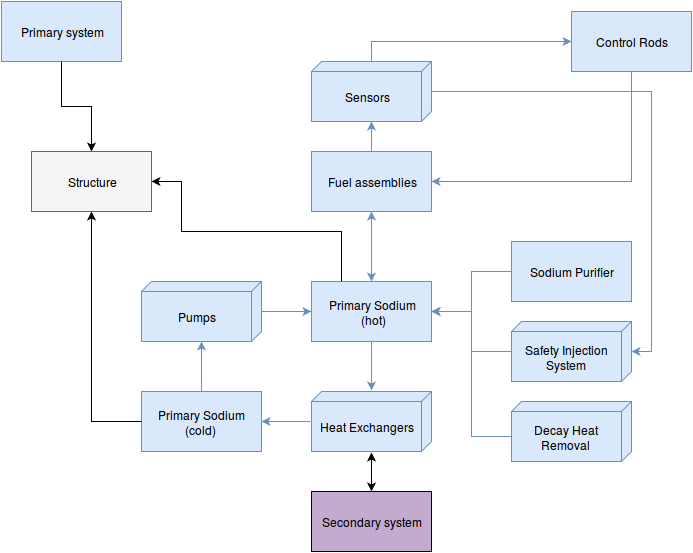
\includegraphics[height=0.6\textheight]{fig04/Primary_system}
	\mycaption[Reliability Block Diagram for the primary system]{Reliability Block Diagram for the primary system}
	\label{fig:rbd_primary_ex}
\end{figure}


\section{Failure Modes and Effects Analysis}
\label{sec:fmea}

Failure Modes and Effects Analysis is a method that ultimately allows designers to identify weaknesses in their systems, by taking into account the probability of a failure to occur ($P$), the severity of the consequences on the system ($S$) and the detectability ($D$). Let us first define these different factors.

\begin{description}

\item[Probability (P)]
On a scale from 0 to 10, this represents the probability of the given failure happening in the considered component, 1 being almost never and 10 being all the time.

\item[Severity (S)]
On a scale from 0 to 10, this represents the consequence of the component failure on the whole system, 0 being no consequence and 10 being catastrophic failure.

\item[Detectability (D)]
On a scale from 0 to 10, this represents the probability to detect the failure and to fix or mitigate the effects, 0 being easy detection and repair and 10 being no possible detection nor action.

\end{description}

Those three factors give the designers a score, the \gls{rpn}, for each identified potential failure throughout the system.

\begin{equation}
RPN = P * S * D
\end{equation}

The designers can then estimate the need for corrections from the highest impacting failure to the lowest. Important shortcomings of this method are to be noted~\cite{liu2013}. It heavily depends on the designers producing the analysis, and their biases (wishful thinking, knowledge, background, ...). Moreover, it can basically only take into account regular failures, that have happened before, and is not adequate for identifying possible "Black Swan" events. It is also not applicable to an early design stage, and thus can generate costly changes that could have been avoided before the conpetion became too advanced. Additionally, the coherence of the RPN formula has been debated. Indeed, one can see from table~\ref{tab:fmea_risk} and~\ref{tab:fmea_rpn_risk} that the RPN is higher for a (3, 6, 6) (P, S, D)-triplet than for a (2, 7, 7) one, implying that in this specific case, the probability of the event occuring is more important than both the severity and the detectability, which can obviously be contested. This also goes to show the huge impact a optimistic or pessimistic estimation can have on the whole RPN ranking and associated conlusions.

Several other FMEA-based methodologies have been developed over the years, to try and cover the shortcomings of FMEA, some examples being the \gls{fmeca} or the fuzzy rule-based system FMEA~\cite{bowles1995}. If a FMEA is to be performed, it is important for the designers to consider the best FMEA method for their project. A classic FMEA was applied to the case study presented in this paper. Even though it is an imperfect method, it can give, and do give, the designers precious information on a high-level.

This study will present a FMEA performed with relation to risks to the system. In the nuclear industry, this is the main one, since it directly impacts communication to the public.

Another FMEA could have been performed with relation to reliability, most useful to the plant operators. The major parameter impacted betwen the two different analyses is the severity. For example, the loss of a generator might be given a 8 on the 10-points scale in the "reliability" study, yet only a 1 in the "risk" study.

This categorization was chosen not to be explicited in details in this paper for clarity reasons. The risk FMEA englobes the reliability ones, with of course a different emphasis.

Follwoing the literature found on the subject~\cite{garcia2013}, the reference tables giving the meaning of each 10-point scale for the Probability, Severity (risk-oriented and reliability-oriented for information) and Detectability parameters score are displayed respectively in tables~\ref{tab:probability},~\ref{tab:severity_risk},~\ref{tab:severity_reliability} and~\ref{tab:detectability}.


\begin{table}[!htb]
    \centering
        \begin{tabular}{ ccc }
        \hline
        Probability & Index & Probability estimate \\ \hline\hline
        \multirow{2}{*}{Inevitable} & 10 & $\geq 0.5$\\
                                    & 9  & $0.1$ \\
        \multirow{2}{*}{Frequent}   & 8  & $0.05$\\
                                    & 7  & $0.02$ \\
        \multirow{3}{*}{Occasional}   & 6  & $0.01$\\
                                    & 5  & $0.005$ \\
                                    & 4  & $0.001$ \\
        \multirow{2}{*}{Minor}   & 3  & $0.0005$\\
                                    & 2  & $0.0001$ \\
        Exceptionally & 1  & $< 0.0001$ \\
                                     
        \end{tabular}
        \caption{Probability index}\label{tab:probability}
\end{table}

\begin{table}[!htb]
    \centering
        \begin{tabular}{ cp{10cm}c }
        \hline
        Severity & Characteristics & Index \\ \hline\hline
        Very high  & The effect can affect both the safety and operation, as the environment, potentially causing damage to property or persons and/or breaking any laws.  & 9 and 10 \\
        High       & Reductions in the power level of the plant and/or weakening the plant safety.  & 7 and 8 \\
        Moderate   & Reduce the system efficiency, generating work stresses which lead the plant to operate in level of risk over of the one in normal condition.  & 4, 5 and 6 \\
        Minor      & The failure effects don't interfere in the plant operation, but reduce shortly the system performance.  & 2 and 3 \\
        Remote     & The failure effect is almost not perceived.  & 1 \\
                                     
        \end{tabular}
        \caption{Detectability index for a risk-centered method}\label{tab:severity_risk}
\end{table}

\begin{table}[!htb]
    \centering
        \begin{tabular}{ cp{10cm}c }
        \hline
        Severity & Characteristics & Index \\ \hline\hline
        Very high  & The effect can affect the operation, potentially causing damage to property or persons and/or breaking any laws. Off-grid time.  & 9 and 10 \\
        High       & Reductions in the power level of the plant.  & 6, 7 and 8 \\
        Moderate   & Reduce the system efficiency, generating work stresses.  & 5 \\
        Low        & The failure effects don't interfere in the plant operation, but reduce shortly the system performance.  & 3 and 4 \\
        Minor      & The failure effect is almost not perceived.  & 2 \\
        Remote     & The failure effect is not perceived on the plant power generation.  & 1 \\
                                     
        \end{tabular}
        \caption{Detectability index for a reliability-centered method}\label{tab:severity_reliability}
\end{table}

\begin{table}[!htb]
    \centering
        \begin{tabular}{ ccc }
        \hline
        Detectability & Index & Detectability estimate \\ \hline\hline
        Very high                   & 1  & 86\% to 100\% \\
        \multirow{2}{*}{High}       & 2  & 76\% to 85\% \\
                                    & 3  & 66\% to 75\% \\
        \multirow{3}{*}{Moderate}   & 4  & 56\% to 65\% \\
                                    & 5  & 46\% to 55\%\\
                                    & 6  & 36\% to 45\% \\
        \multirow{2}{*}{Low}        & 7  & 26\% to 35\% \\
                                    & 8  & 13\% to 25\%\\
        \multirow{2}{*}{Minor}      & 9  & 6\% to 15\% \\
                                    & 10 & 0\% to 6\% \\
                                     
        \end{tabular}
        \caption{Detectability index}\label{tab:detectability}
\end{table}

An extensive -- yet incomplete, by essence of the method -- FMEA has been performed on the system at hand. The failure modes, causes and (P, S, D)-triplets can be seen in table~\ref{tab:fmea_risk} and the RPN and mitigation actions in table~\ref{tab:fmea_rpn_risk}.

The range of values obtained using the aforementionned reference tables for the different parameters goes from 4 for a large breach of the core catcher to 400 for an erroneous signal from every detectors. The perceived failure modes with the greatest RPN number have been selected and are presented in tables~\ref{tab:excerpt_fmea} and~\ref{tab:excerpt_rpn_fmea}.

\begin{table}[!htb]
    \centering
        \begin{tabular}{ccp{4cm}p{4cm}ccc}
            \hline
            ID & Component & Failure & Cause & $P$ & $S$ & $D$ \\ \hline \hline
            8.1 & \multirow{1}{3cm}{Detectors}  & Wrong signal from all & Electronic components & 5 & 8 & 10 \\ \hline
            11.2 & \multirow{1}{3cm}{Main vessel} & Small breach & Aggression & 3 & 10 & 10 \\ \hline
            12.4 & \multirow{2}{3cm}{Safety vessel}  & Large breach & Aggression & 3 & 9 & 10 \\ 
            12.2 &                                   & Small breach & Aggression & 3 & 8 & 10 \\
        \end{tabular}
        \caption{Excerpt from Table\ref{tab:fmea_risk} presenting the (P, S, D)-triplet for the perceived most severe failure modes}\label{tab:excerpt_fmea}
\end{table}


\begin{table}[!htb]
    \centering
        \begin{tabular}{ccp{10cm}}
            \hline
            ID & RPN & Mitigation \\ \hline\hline
            8.4 & 400  & Calibrate the detectors frequently, use different kind, use other ways to determine reactor power output \\
            11.2 & 300 & Good material and large width, external defense \\
            12.4 & 270 & Good material and large width, external defense \\
            12.2 & 240 & Good material and large width, external defense \\
        \end{tabular}
        \caption{Excerpt from Table\ref{tab:fmea_rpn_risk} presenting the RPN and possible mitigation strategy for the perceived most severe failure modes}\label{tab:excerpt_rpn_fmea}
\end{table}

One of the main issues with the FMEA, as discussed previously, is the subjectivity of the data, highly dependable on the designer's experience and expertise. All the different systems (electronic, electric, mechanical, nuclear, ...) should be analyzed, and a large panel of experts is thus needed. The author of this paper applied enegineering training and experience to deduce some of the (P, S, D)-triplets. The principal strength of this method resides in its simplicity and its capability to quicjly give the designer an idea of potential problems to be fixed within the system.

